% Chapter 1

\chapter{Giới thiệu} % Main chapter title

\label{Chapter1} % For referencing the chapter elsewhere, use \ref{Chapter1} 

%----------------------------------------------------------------------------------------

% Define some commands to keep the formatting separated from the content 
\newcommand{\keyword}[1]{\textbf{#1}}
\newcommand{\tabhead}[1]{\textbf{#1}}
\newcommand{\code}[1]{\texttt{#1}}
\newcommand{\file}[1]{\texttt{\bfseries#1}}
\newcommand{\option}[1]{\texttt{\itshape#1}}

%----------------------------------------------------------------------------------------

\section{Tổng quan}
Cùng với sự phát triển của đô thị hoá, giao thông, đặc biệt là ùn tắc giao thông trở thành vấn đề nan giải đối với tất cả những quốc gia đông dân trên thế giới, và Việt Nam cũng không ngoại lệ.

Xét trên địa bàn thành phố Hồ Chí Minh, trước kia ùn tắc chỉ xảy ra ở một số điểm cửa ngõ vào giờ cao điểm thì hiện nay, tình trạng này càng trở nên nghiêm trọng, ở nhiều nút giao thông và không theo một quy luật cố định, ảnh hưởng tiêu cực trực tiếp đến người dân \cite{VOV}.

\begin{figure}[H]
\centering
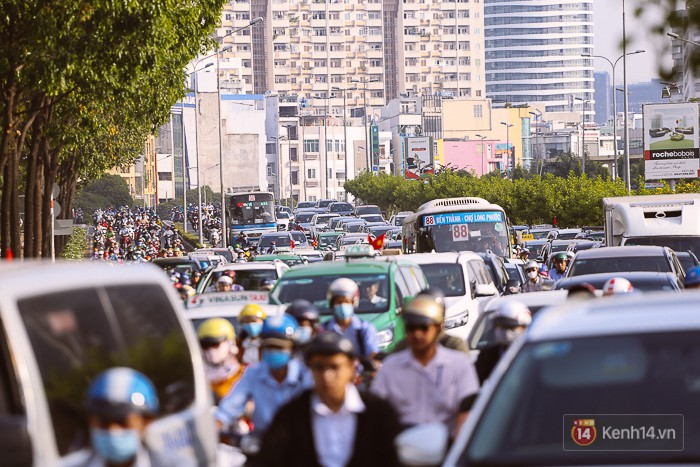
\includegraphics[width=1.0\textwidth]{Traffic_Report/images/image01.jpg}
\caption{Kẹt xe trên đường Nguyễn Hữu Cảnh hướng Bình Thạnh về Quận 1}\label{}
\end{figure}

Có nhiều nguyên nhân gây ra ùn tắc giao thông:
\begin{itemize}
    \item Về mặt cơ sở hạ tầng: không đủ nguồn cung về đường sá để đáp ứng lưu lượng giao thông lớn; chất lượng thi công không đảm bảo; đèn giao thông không đồng bộ; phân luồng bất hợp lý... \cite{MNN}
    \item Về mặt con người: công tác quản lý đường, giải quyết tai nạn giao thông còn nhiều bất cập; ý thức người tham gia giao thông yếu kém, chưa có trách nhiệm về an toàn giao thông...
\end{itemize}
Mỗi nguyên nhân trên có thể đưa ra nhiều giải pháp khắc phục. Tuy nhiên nhìn chung, việc giải quyết đòi hỏi thời gian lâu dài, cần sự kết hợp của cả chính quyền và người dân. Đây thật sự là một thách thức lớn mà rất ít thành phố lớn trên thế giới có thể giải quyết được, huống hồ là một nơi với mật độ dân cư đông đúc và phức tạp như thành phố Hồ Chí Minh.

Bản chất của quá trình ùn tắc là sự tập trung một lượng lớn phương tiện giao thông vào một đoạn đường với diện tích bề mặt không đủ rộng, dẫn tới sự chen lấn và trì trệ sự di chuyển của các phương tiện \cite{MUTC}. Từ đó có thể thấy được, dù giải quyết triệt để ùn tắc giao thông là vô vùng khó khăn, người dân vẫn có thể chủ động tránh ùn tắc bằng cách lựa chọn tuyến đường có mật độ phương tiện thấp.

Với hướng tiếp cận trên, cần thiết xây dựng một hệ thống thu thập dữ liệu giao thông, xử lý và đưa ra cho người dùng thông tin về giao thông theo thời gian thực, có khả năng dự báo tình trạng giao thông để người dùng chủ động phòng tránh ùn tắc, định hướng lộ trình hợp lý.

\section{Nhiệm vụ đề cương luận văn}
Nhiệm vụ đề cương luận văn gồm có:
\begin{enumerate}
    \item Nghiên cứu, kiểm tra độ tin cậy, lựa chọn và thu thập dữ liệu dựa trên các nguồn có sẵn như Here Maps, Smart BK Traffic, dữ liệu thu thập từ cộng đồng (crowdsourcing)...
    \item Bước đầu xây dựng ứng dụng web hiển thị dữ liệu giao thông lên bản đồ cung cấp từ OpenStreetMap, từ đó có thể đánh giá mức độ ùn tắc giao thông trên các tuyến đường trên địa bàn thành phố Hồ Chí Minh.
\end{enumerate}

\section{Các nghiên cứu liên quan}
Trước tình hình giao thông ngày càng đông đúc, phức tạp tại các thành phố lớn, trong đó có thành phố Hồ Chí Minh. Nhiều biện pháp, nghiên cứu cũng được đề ra để giải quyết vấn đề nhức nhối này \cite{FSPPM}. Cũng đã có rất nhiều báo cáo khoa học và nghiên cứu đề xuất giải pháp giải quyết bài toàn này. Tuy nhiên, phần lớn các báo cáo khoa học hay nghiên cứu đều tập trung vào cách thu thập dữ liệu về luồng giao thông bằng những thiết bị cảm biến, nhận diện bằng hình ảnh, video và đưa ra dự đoán \cite{VEGV} \cite{RTD}. Các phương pháp này đều cần một hệ thống cơ sở hạ tầng hiện đại, tiên tiến để thu thập dữ liệu và phân tích sau đó đưa ra kết quả nhằm mục đích nghiên cứu lâu dài.

Ở Việt Nam, cụ thể là thành phố Hồ Chí Minh, sở giao thông thành phố cũng đã đưa ra ứng dụng \cite{VOVAPP} cho phép người dân xem xét dòng giao thông hiện tại hoặc xem các hình ảnh trực tiếp của tuyến đường có gắn camera. Đồng thời, nhóm nghiên cứu Intelligent Transport System tại Đại học Bách Khoa thành phố Hồ Chí Minh cũng thực hiện một trang web \cite{HCMUT} thông báo tình trạng giao thông từ GPS của các tuyến xe bus tương tự các hệ thống trên đem lại các kết quả khả quan.

Bên cạnh đó, còn có một hướng đi khác là thu thập dữ liệu từ cộng đồng (crowdsourcing) đã được nhiều tổ chức, công ty \cite{16} sử dụng hiệu quả khi tích hợp vào các hệ thống của mình. Điển hình là trận động đất ở Haiti năm 2010, hệ thống Ushahidi hoạt động dựa trên mô hình crowdsourcing đã hoạt động rất hiệu quả trong việc thu thập dữ liệu, phân tích và đưa ra những chỉ dẫn trực tiếp cho các tình nguyện viên để sơ tán, di tản người dân Haiti về khu vực an toàn \cite{23} \cite{24}.

Kế thừa từ những nghiên cứu, kết quả đã đạt được ở trên. Nhóm nghiên cứu mong muốn đưa ra hệ thống kết hợp dữ liệu lấy được từ các hệ thống giao thông sử dụng dữ liệu GPS, đồng thời xây dựng nguồn dữ liệu crowdsourcing bằng ứng dụng di động và các phương pháp khuyến khích chia sẻ dữ liệu cũng như xác thực tính đúng đắn của dữ liệu để đưa ra những dự đoán tình hình giao thông một cách hoàn thiện và chính xác nhất. 